\chapter{Результаты расчетов}

$$\hat{\mu} = 1.84$$
$$S^2 = 1.15$$

$$\overline{\mu}(\vec{x}) = 2.00$$
$$\underline{\mu}(\vec{x}) = 1.67$$

$$\overline{\delta^2}(\vec{x}) = 1.45$$
$$\underline{\delta^2}(\vec{x}) = 0.94$$

\begin{figure}[h]
  \centering
  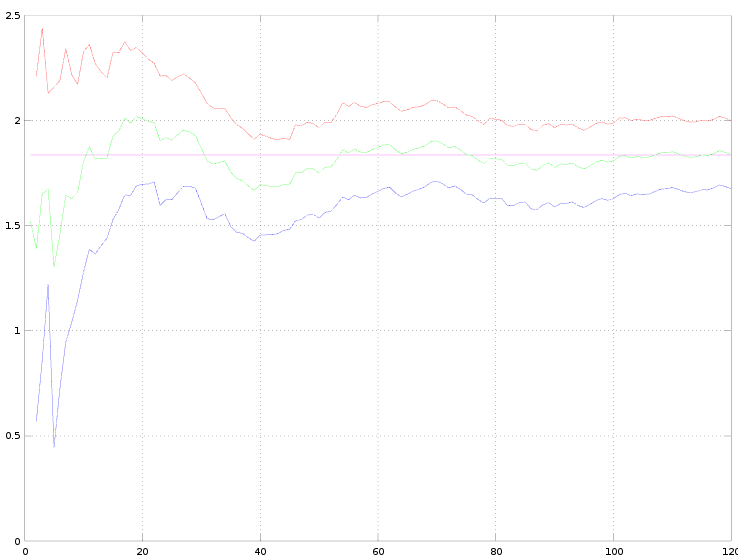
\includegraphics[width=\textwidth]{pic1.png}
  \caption{Прямая $y = \hat{\mu}(\vec{x}_N)$ и графики функций $y = \hat{\mu}(\vec{x}_n)$, $y = \underline{\mu}(\vec{x}_n)$, $y = \overline{\mu}(\vec{x}_n)$ как функций объема n выборки, где n изменяется от 1 до N}
\end{figure}

\begin{figure}[h]
  \centering
  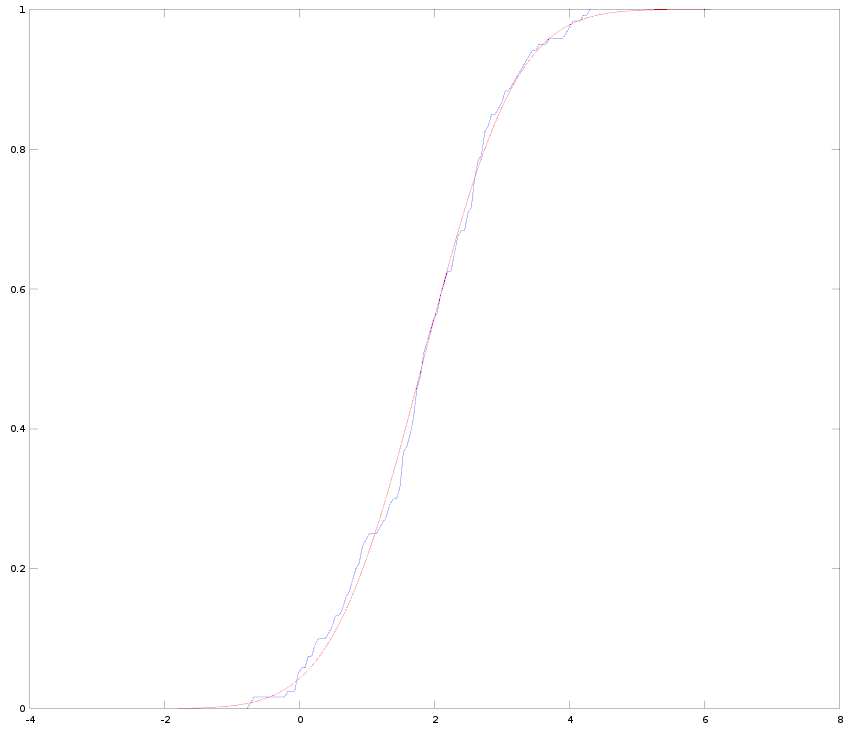
\includegraphics[width=\textwidth]{pic2.png}
  \caption{Прямая $z =  S^2(\vec{x}_N)$ и графики функций $z = S^2(\vec{x}_n)$, $z = \underline{\sigma^2}(\vec{x}_n)$, $z = \overline{\sigma^2}(\vec{x}_n)$ как функций объема n выборки, где n изменяется от 1 до N}
\end{figure}